При разработке сервиса было поставлено несколько целей:
\begin{itemize} 
\item Тестирование программного комплекса;
\item Проведение тренировочной игры для команды;
\item Упаковка сервиса в <<стартовый набор>> для ознакомления.
\end{itemize}

Сервис писался на языке Python с использованием базы данных MongoDB и микрофреймворка Flask.

Тестирование платформы заключалось в тестировании следующий функций:
\begin{itemize} 
\item Работа чекера (методы check, get, put);
\item Работа модуля сдачи флагов;
\item Работа платформы в условиях медленного <<ответа>> сервиса.
\end{itemize}

Смысл сервиса состоит в том, что при регистрации пользователь указывает свою электронную почту, пароль и имя.
Если пользователь уже регистрировался, то он просто входит в систему, при условии, что логин и пароль  совпадают. Далее пользователь видит приветственное сообщение в формате <<Привет, <имя пользователя>>>

\begin{figure}[ht!]
\center{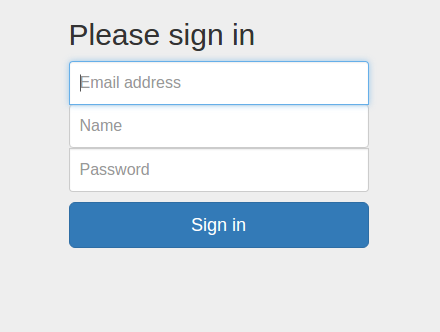
\includegraphics[width=0.5\linewidth]{eco/images/dima_main.png}}
\caption{Главная страница сервиса}
\end{figure} 

Несмотря на простоту сервиса, в нем содержится несколько уязвимостей:
\begin{itemize} 
\item Открытый порт БД (незащищенный паролем);
\item Уязвимость в данных cookie;
\end{itemize}

